%% -*- coding: utf-8 -*-
\documentclass[12pt,pagesize,paper=192mm:108mm,landscape]{scrbook} 
%1920x1080 1280x720
\areaset[current]{192mm}{108mm}
\usepackage{calc}
\usepackage[T2A]{fontenc}
\usepackage[utf8]{inputenc}
\usepackage[english,russian]{babel}
\usepackage{microtype}
\usepackage{misccorr}
\usepackage{cmap}
%\usepackage[unicode=true]{hyperref}
\usepackage{graphicx}
\usepackage{amssymb}
\usepackage{amsmath}
%\usepackage{srcltx}
\usepackage{textcomp}
\usepackage{xspace}
%научные символы и смайлики \smiley \frownie
\usepackage{wasysym}
\usepackage{ccicons}
\begin{document}
\begin{titlepage}
  \vspace*{-0.5em}
  \begin{center}    
    \hspace*{3em}
    \begin{minipage}[t]{1.5em}
      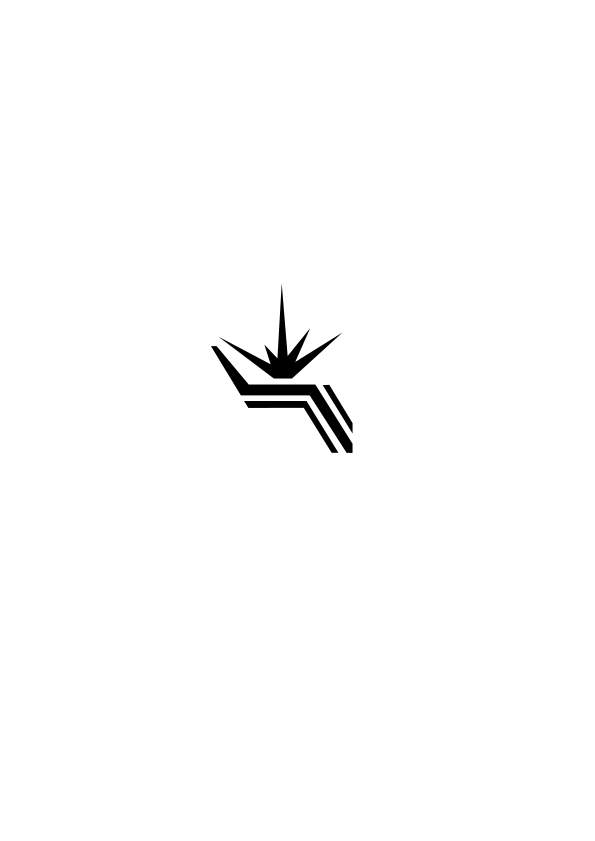
\includegraphics[width=\textwidth]{../BINP-logo}
    \end{minipage}\hfill
    \begin{minipage}{0.115\linewidth}
    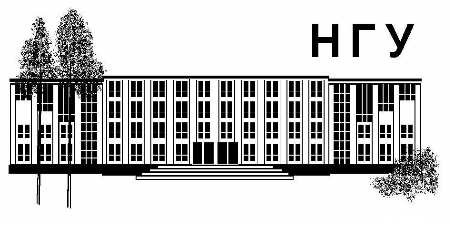
\includegraphics[width=\textwidth]{../NSU-logo}
    \end{minipage}
    \hfill
    \hspace*{4.5em}

    Кафедра теоретической физики физического факультета НГУ
    \medskip

    \Large
    Профессор Грабовский А.\,В.
    \smallskip

    \huge
    \textbf{Стандартная модель}
    \smallskip

    \Large
    Лекция № 2
    \vfill

    \normalsize
    \begin{minipage}{0.85\linewidth}
      Юкавское взаимодействие поля Хиггса и фермионов. Массы
      фермионов. Базис взаимодействия и массовый базис для фермионов
      трех поколений. Переход в массовый базис. Инвариантность
      нейтральных токов относительно перехода между
      базисами. Инвариантность заряженного лептонного тока для нулевых
      масс нейтрино. Смешивание поколений кварков. Матрица
      Кабиббо"--~Кобаяши"--~Маскава $V$ в различных представлениях. Количество
      свободных параметров в матрице СКМ. Угол Кабиббо, треугольник
      унитарности, инвариант Ярлског.
    \end{minipage}
    \vfill

    \normalsize \ccbysa\hspace{0.5em}  Новосибирск 2024
  \end{center}
\end{titlepage}
\end{document}
